% Please use the skeleton file you have received in the
% invitation-to-submit email, where your data are already
% filled in. Otherwise please make sure you insert your
% data according to the instructions in PoSauthmanual.pdf
\documentclass{PoS}

\title{Higgs boson searches beyond the Standard Model}

\ShortTitle{Short Title for header}

\author{\speaker{Claudio Caputo}\thanks{A footnote may follow.}\\
        Universit\'a degli Studi di Bari, Istituto Nazione di Fisica Nucleare\\
        E-mail: \email{claudio.caputo@cern.ch}}

\author{Paolo Francavilla\thanks{This work is partially supported by the ILP
LABEX (under reference ANR-10-LABX-63 and ANR-11-IDEX-0004-02).}\\
        Laboratoire de Physique Nucl\'eaire et de Hautes Energies and Institute Lagrange de Paris,\\
        E-mail: \email{paolo.francavilla@cern.ch}}

\abstract{The discovery of the a scalar particle at the Large Hadron Collider (LHC) is one of the major achivements by the ATLAS and CMS collaborations. Important questions on the nature of this new boson and on possible extensions of the scalar sector of the Standard Model have been addressed by both the ATLAS and CMS collaborations with a vast variety of searches performed  at a centre-of-mass energy of 7 TeV and 8 TeV (LHC Run 1). Thanks to the first LHC collision at a centre-of-mass energy of 13 TeV (LHC Run 2), new searches which go beyond the Run 1 reach, have been performed by the LHC collaborations. Among them we describe the searches for  $A/H\rightarrow\tau\tau$ and $H\rightarrow hh$ in this proceeding. }

\FullConference{VII Workshop italiano sulla fisica pp a LHC\\
		16-18 Maggio 2016\\
		Pisa, Italy}


\begin{document}

\section{Introduction}
Following the discovery of a scalar particle at the Large Hadron Collider (LHC), an important
question is whether this is the Standard Model (SM) Higgs boson or part of an extended Higgs
sector. One interesting approach to answer this question is to search for additional scalars,
whose observation could confirm existence of an extended Higgs sector.
For the first LHC collision data provided at a centre-of-mass energy of 13 TeV and recorded
by the ATLAS and CMS detectors, the collaborations have performed many searches that are
motivated by a variety of models beyond the SM. The simplest extensions of the SM involve the
addition of an additional singlet or doublet field, known as Electroweak Singlet Models (EWS)
and Two-Higgs-Doublet Models (2HDM), respectively. Many searches are motivated by these
extensions and benchmarks within specific related models, such as the Minimal Supersymmetric
Standard Model (MSSM). The MSSM in a particular benchmark scenario is completely
determined by two parameters, the mass of one of the Higgs bosons and the ratio of the vacuum
expectation values, tan$\beta$.
This proceeding will detail the wide variety of new searches performed with the 13 TeV
data, which are performed with an integrated luminosity of 3.2 fb$^{−1}$ and up to 2.8 fb$^{−1}$ with the
ATLAS and CMS detectors, respectively. Several recent results with the 8 TeV dataset were
also presented, but will not be discussed here.
.


\section{Search for neutral  Higgs bosons $H/A \rightarrow \tau\tau$}
For heavy neutral Higgs in models with extended Higgs sectors, such as the MSSM, the decay
to two $\tau$ leptons is dominant at high masses and values of tan$\beta$. The ATLAS collaboration has
performed a search for neutral Higgs bosons decaying to $\tau$ leptons using an integrated luminosity
of 3.2 fb$^{−1}$. The search is performed in two channels, where one $\tau$ decays leptonically and the
other hadronically ($\tau_{\rm lept}$$\tau_{\rm had}$) and where both $\tau$ leptons decay hadronically ($\tau_{\rm had}$$\tau_{\rm had}$) .
In the $\tau_{\rm had}$$\tau_{\rm had}$ channel, multi-jet events form the dominant background, and they are estimated
using a data-driven fake-factor method. Events from other processes with a jet misidentified
as a $\tau_{\rm had}$, such as W+jets and top-quark backgrounds, are taken from simulation and
corrected using fake rates measured from data. Events with correctly identified $\tau_{\rm had}$ are taken
from simulation, with some data-driven corrections to the normalization.
In the $\tau_{\rm lept}$$\tau_{\rm had}$, backgrounds from all processes that involve jets misidentified as $\tau_{\rm had}$
are estimated simultaneously in a data-driven fake-factor method that takes into account the
fractional contribution of the dominant background processes of W+jets and multi-jets. Events
with electrons misidentified as a $\tau_{\rm had}$ are suppressed in the electron channel with a veto on the
visible mass of the $\tau_{\rm had}$ and lepton of the Z boson mass window, $80~{\rm GeV} < m_{\rm vis} < 110~{\rm GeV}$.
The remaining backgrounds are corrected with a data-driven scale factor derived within the Z boson mass window. Backgrounds with a correctly identified $\tau_{\rm had}$ are taken from simulation.
In both channels, the final discriminating variable is 
The final result is provided both as a limit on the cross section times branching ratio as well
as a model-dependent limit on various MSSM benchmark models. The sensitivity exceeds the
8 TeV result for $m_{H} >$ 750 GeV. The limits for all channels combined are shown in Figure 2
for the gluon fusion and b-associated production methods, with the separate expected limits for
the $\tau_{\rm lept}$$\tau_{\rm had}$ and $\tau_{\rm had}$$\tau_{\rm had}$ channels overlaid.

\newpage
\clearpage
\section{Search for Higgs boson pair production}
\label{ref:HHProduction}

The Higgs boson pair production could be use to investigate both the SM and the BSM scenarios. 
\\
Searches for \emph{non-resonant} $hh$ production give information on the trilinear coupling present in the SM Higgs potential fields; the same searches could spot out discrepancies with respect to the SM $\lambda_{hhh}$ introduced by anomalous couplings and new physics.
\\
Similar searches in the \emph{resonant} regime could be used to explore the BSM world; new particles, introduced by extensions in the $\mathcal{L}_{SM}$, could decay in a couple of Higgs SM like boson (Di-Higgs). The experience acquired during the $8 \, TeV$ data taking period at LHC for SM Higgs search is used for seek different final state configuration of the Di-Higgs. 

In this paragraph an overview of the latest \emph{resonant} results, provided by ATLAS and CMS experiment for  $13\, TeV$ collision, will be presented. Both collaboration have produced results with $8\, TeV$ data \cite{HH_ATLAS_8TeV}\cite{HH_CMS_8TeV} 
in many Di-Higgs decay configurations as shown in figure \ref{fig:HH_8TeV_Results}.
 
%%
\begin{figure}[htb]
\centering
	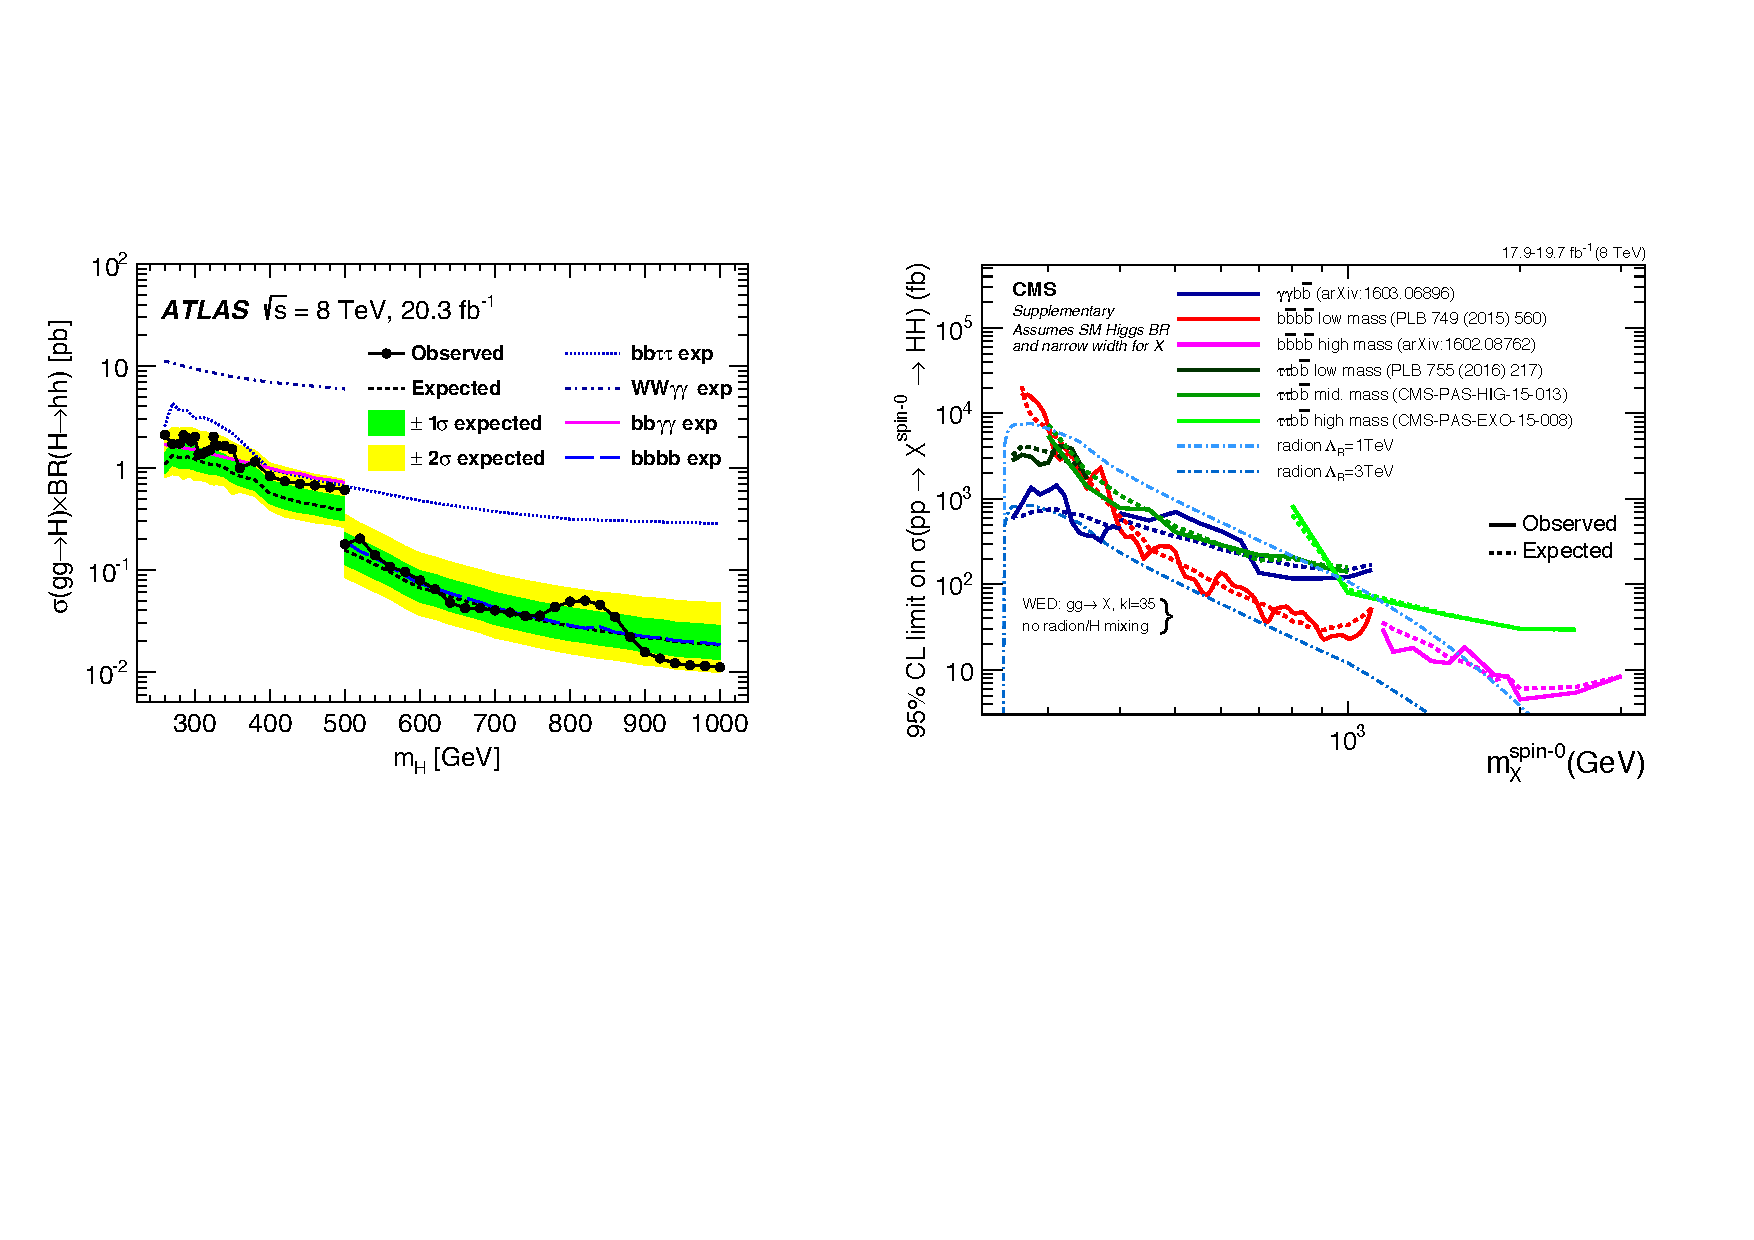
\includegraphics[width=1.0\textwidth, angle=0] {figures/HH_8TeV.pdf}
\caption{(left) ATLAS combination Higgs boson pair production in the $hh\ensuremath{\rightarrow}bb\ensuremath{\tau}\ensuremath{\tau}$, $\ensuremath{\gamma}\ensuremath{\gamma}W{W}^{*}$, $\ensuremath{\gamma}\ensuremath{\gamma}bb$, $bbbb$ channels with $8\,TeV$ data, (right) CMS Observed and expected 95\% CL upper limits on the product of cross section and the branching fraction $\sigma(gg\rightarrow X) \times B(X\rightarrow hh)$ obtained by different analyses assuming spin-0 hypothesis.}
\label{fig:HH_8TeV_Results}   
\end{figure}
%%

\subsection{$H\rightarrow hh \rightarrow bbbb$ channel}
The Higgs boson decay mode in b quarks has the highest branching ratio, this imply that a Di-Higgs final state, with each Higgs dacaying into a b pair, it's the most prominent one between the others. Although search of this kind of final state should take into account the overwhelming multi-jet background, largely produced at hadrons collider.

ATLAS and CMS collaborations analysis scan a mass range $260\, GeV \, < m_{H}  <  3000 \, GeV$, particularly CMS cover from $260\, GeV$ to $1200\, GeV$ and ATLAS from $500\, GeV$ to $3000\, GeV$. Both analysis have different strategy for different $m_H$ ranges: low-mass region ($260\, GeV \, < m_{H}  <  400 \, GeV$), medium-mass ragion ($400\, GeV \, < m_{H}  <  1200 \, GeV$), boosted region ($1200\, GeV \, < m_{H}  <  3000 \, GeV$). The categorisation is chosen to maximise to significance of the analysis. 

The results are shown in figure \ref{fig:HH_bbbb}.
 %%
\begin{figure}[htb]
\centering
	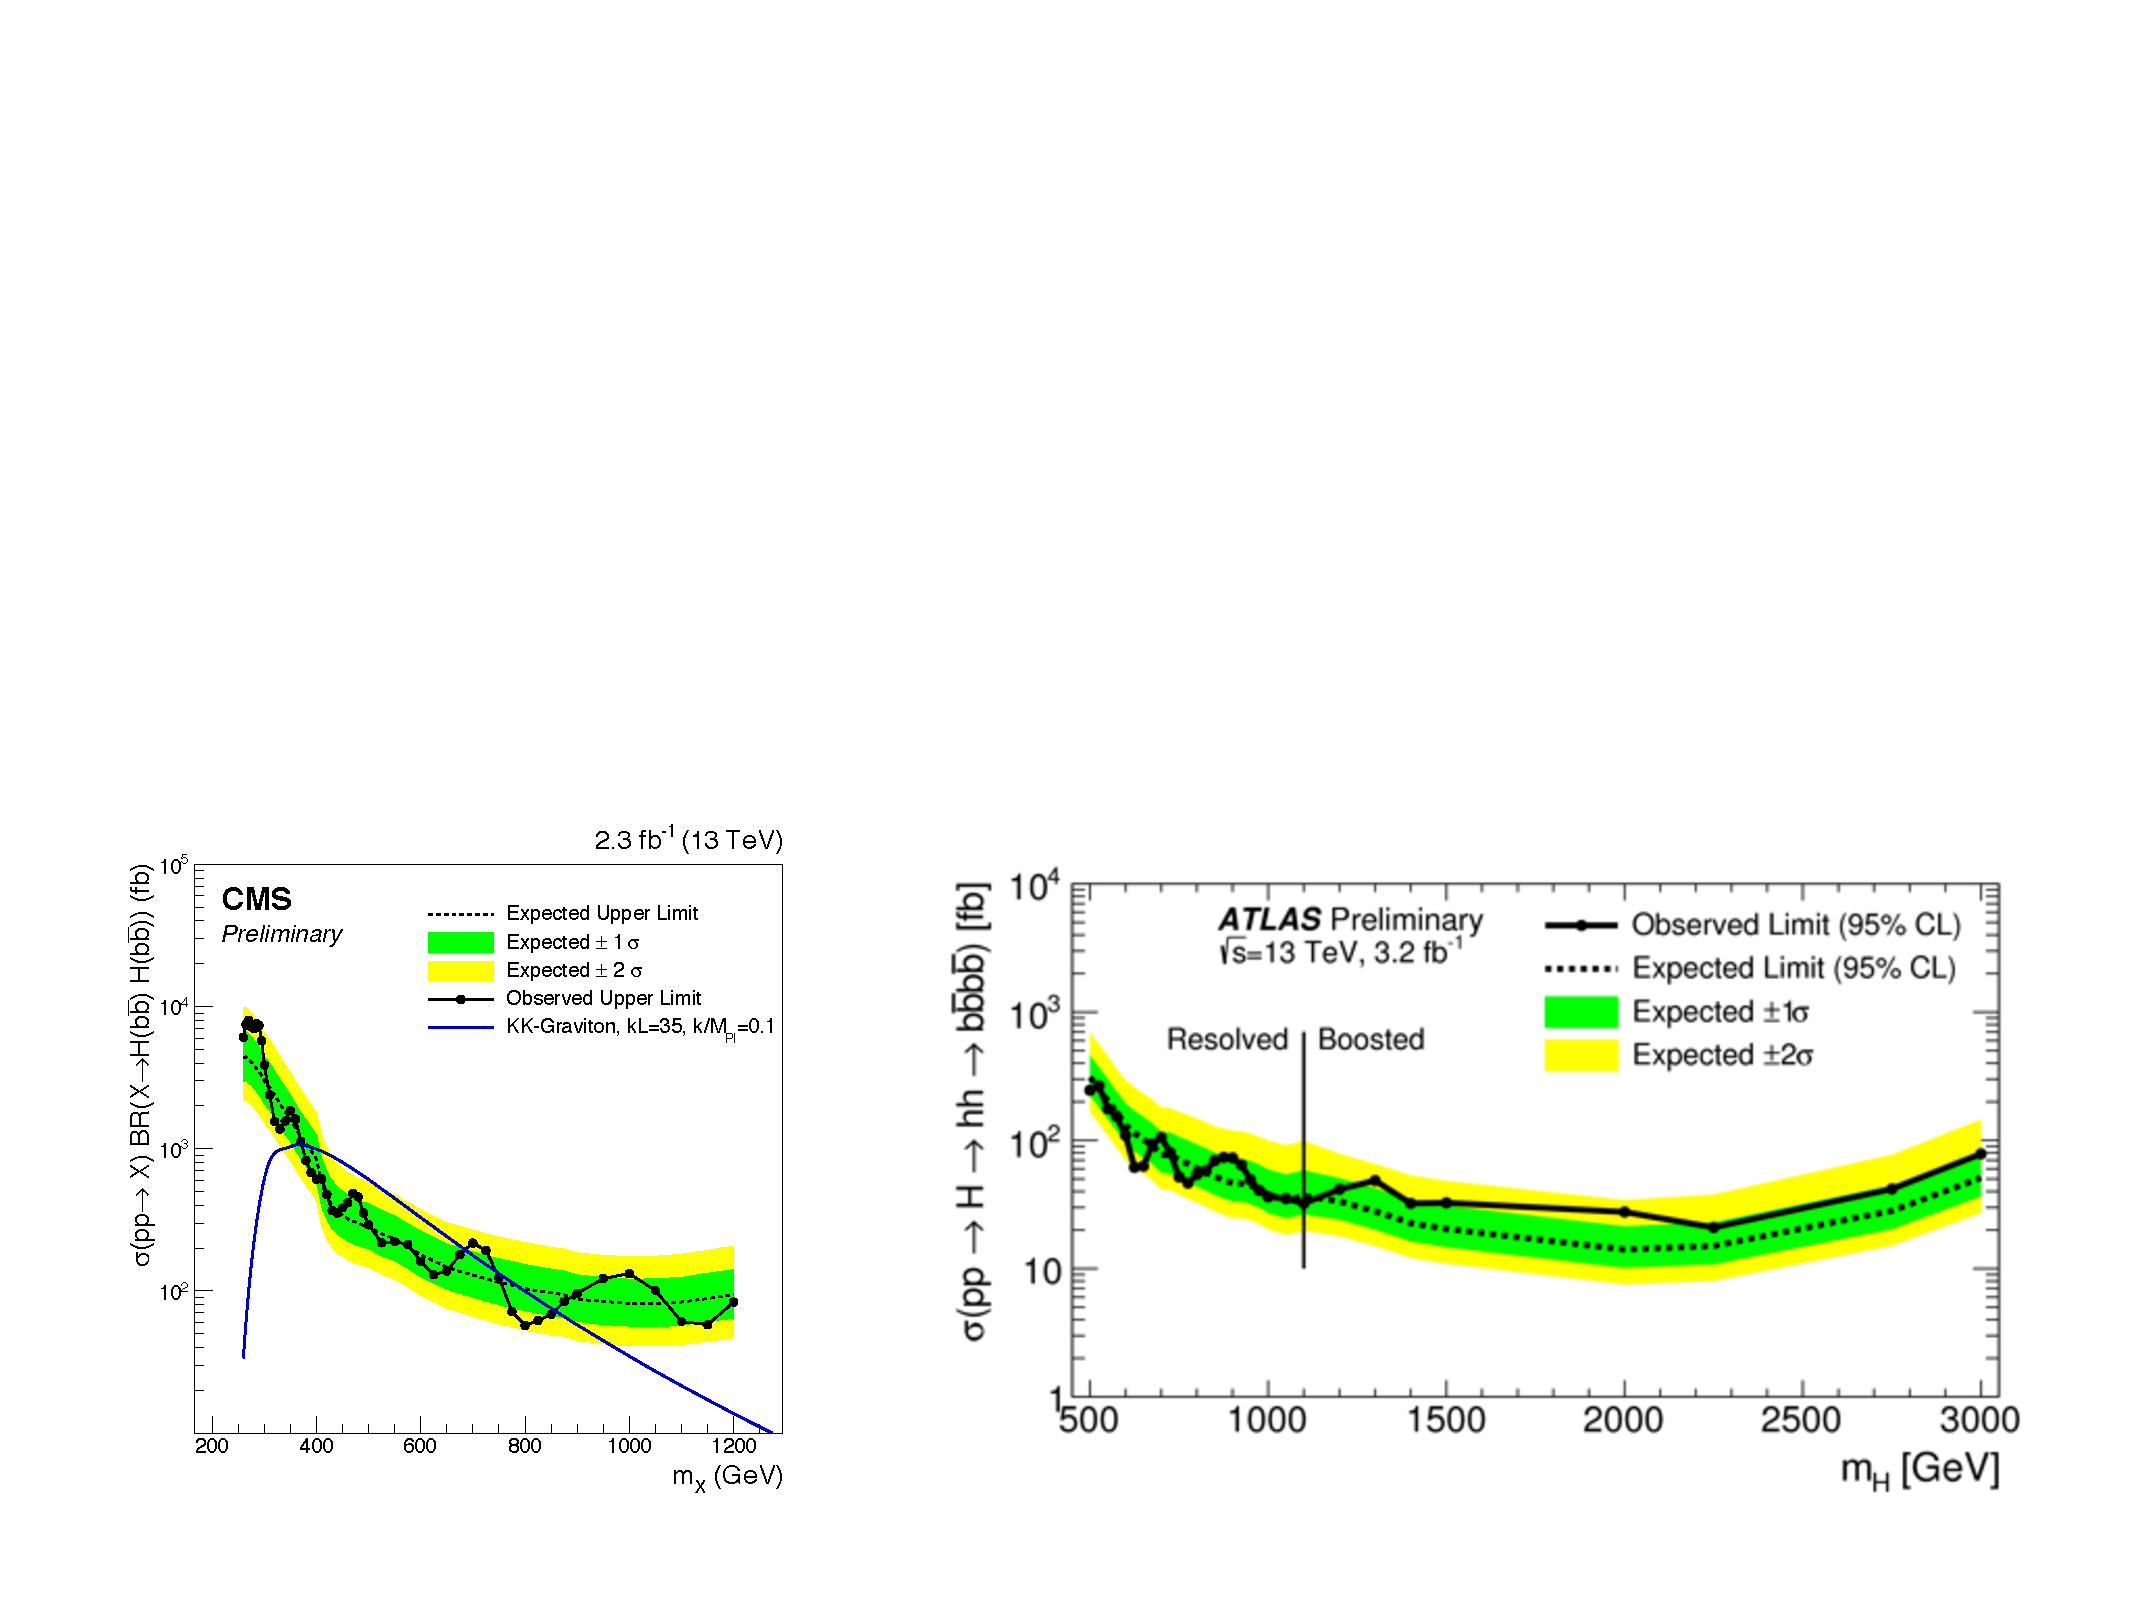
\includegraphics[width=1.0\textwidth, angle=0] {figures/HH_bbbb.pdf}
\caption{(left) CMS: The observed and expected upper limits on the cross section for a spin-2 resonance
$H\rightarrow hh\rightarrow bbbb$ at a 95\% confidence level using data corresponding to an integrated luminosity
of $2.3 fb^{?1}$ at $13 TeV$ using the asymptotic $CL_S$ method, (right) ATLAS: The expected and observed upper limit for $pp\rightarrow H\rightarrow hh\rightarrow bbbb$ with fixed $\Gamma_H = 1 GeV$, at the 95\% confidence level .}
\label{fig:HH_bbbb}   
\end{figure}
%%
 
\subsection{$H\rightarrow hh \rightarrow bb\tau\tau$ channel}
The $bb\tau\tau$ channel can exploit the presence of the $\tau$ leptons to take care of the multi-jet background.

The analysis performed by CMS collaboration scans a $260\, GeV \, < m_{H}  <  900 \, GeV$ and combine three different $\tau\tau$ final state: $\mu\tau_h$, $e\tau_h$ and $\tau_h\tau_h$, where $\tau_h$ stands for the hadronic decays of a $\tau$. 
The finale $m_H$ shape is constructed using a dedicated kinematic fit procedure.

Observed and expected 95\% CL upper limits are shown in figure \ref{fig:HH_bbtt}.


 %%
\begin{figure}[htb]
\centering
	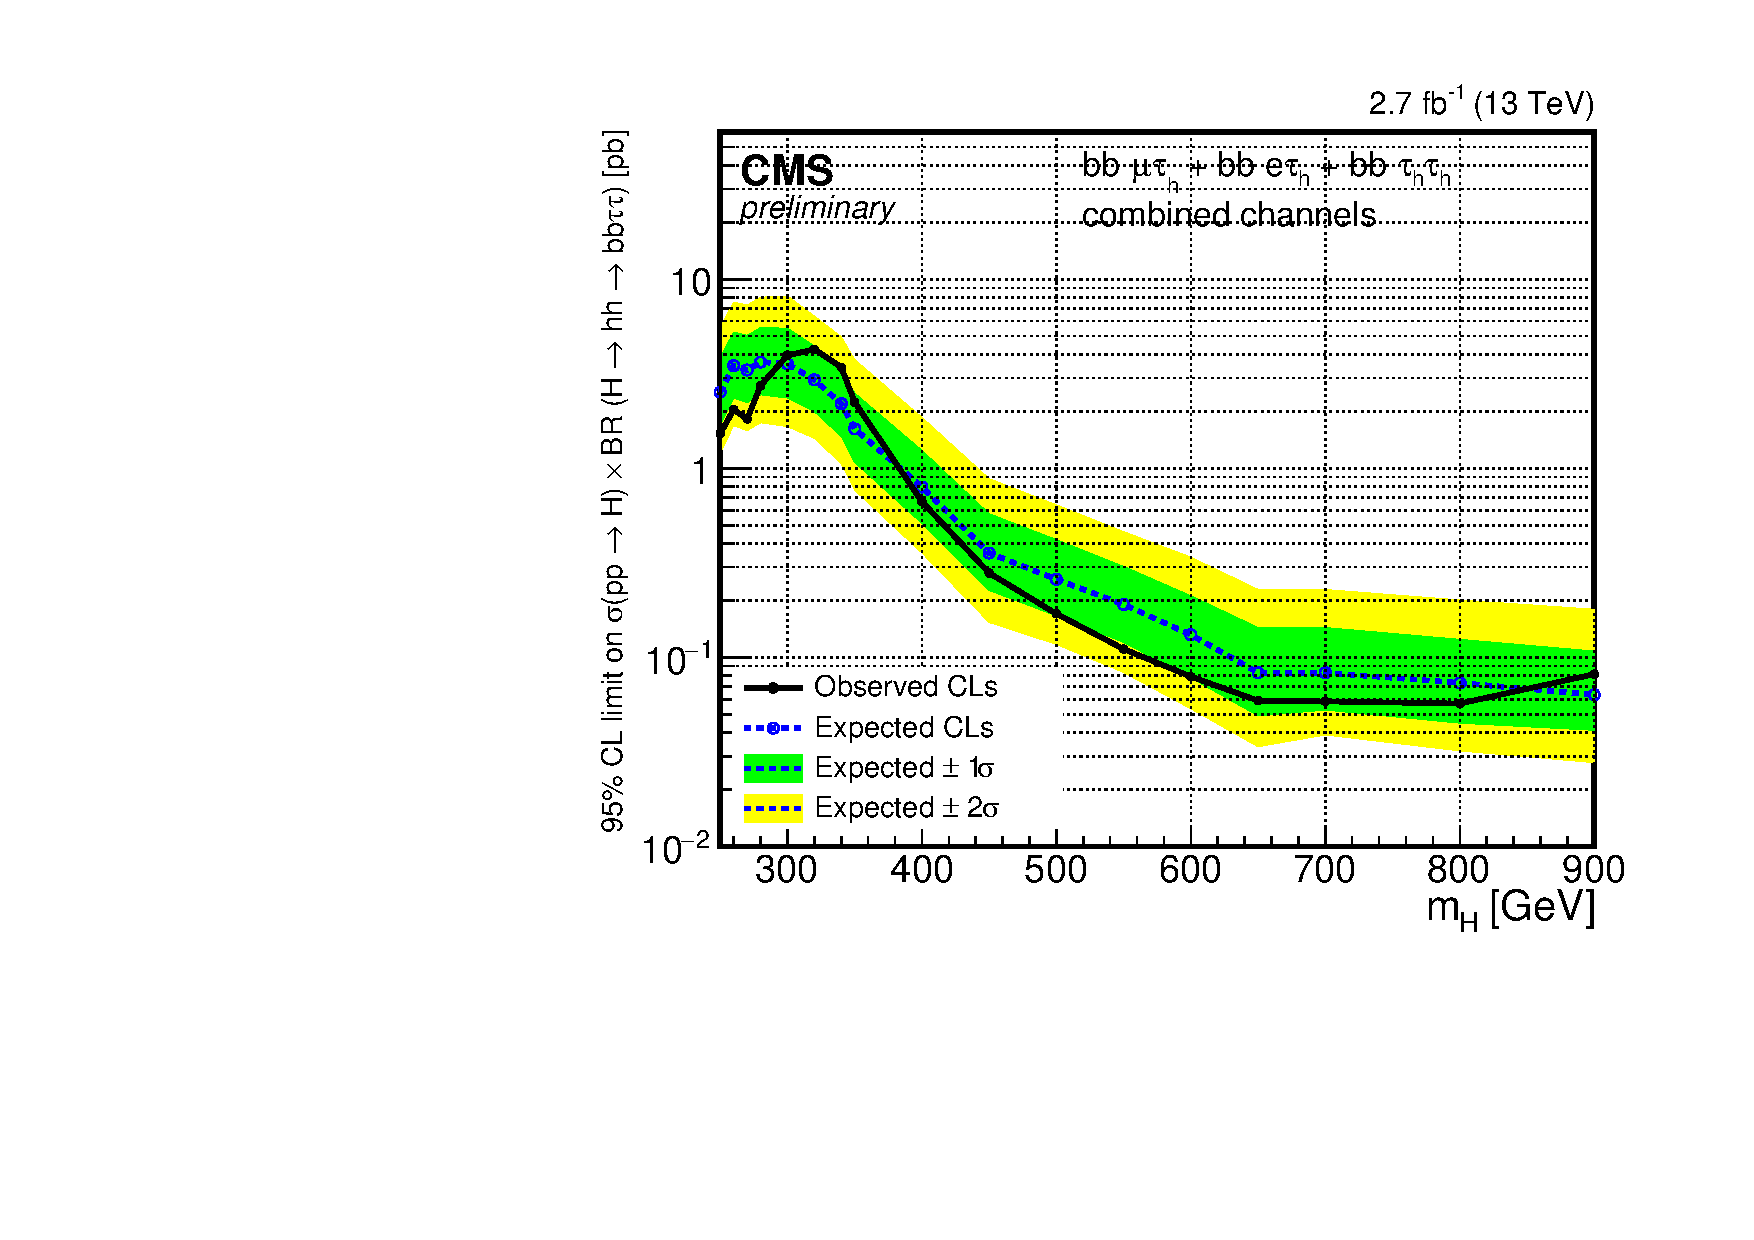
\includegraphics[width=0.7\textwidth, angle=0] {figures/H_hh_bbtautau_CMS_BR.pdf}
\caption{Observed and expected 95\% CL upper limits on $\sigma(pp\rightarrow H) \times BR(H \rightarrow hh \rightarrow bb\tau\tau)$
from the combination of the three channels as a function of the mass of the resonance $m_H$}
\label{fig:HH_bbtt}   
\end{figure}
%%

\subsection{$H\rightarrow hh \rightarrow bbWW$ channel}
The search for resonant Higgs pair production, $H \rightarrow hh$, where one of the h decays as $h\rightarrow bb$, and the other as $H \rightarrow WW \rightarrow l?l?$ (where l is either an electron or a muon) is performed by CMS collaboration using LHC proton-proton collision data at $13\, TeV$. The analysis focuses on the invariant mass distribution of the b-jet pair, searching for a resonant-like excess compatible with the h boson mass in combination with a boosted decision tree discriminant based on kinematic information. The dominant background is tt production with smaller contributions
from Drell-Yan and single top processes. Figure \ref{fig:HH_bbWW} shows the result obtained.

 %%
\begin{figure}[htb]
\centering
	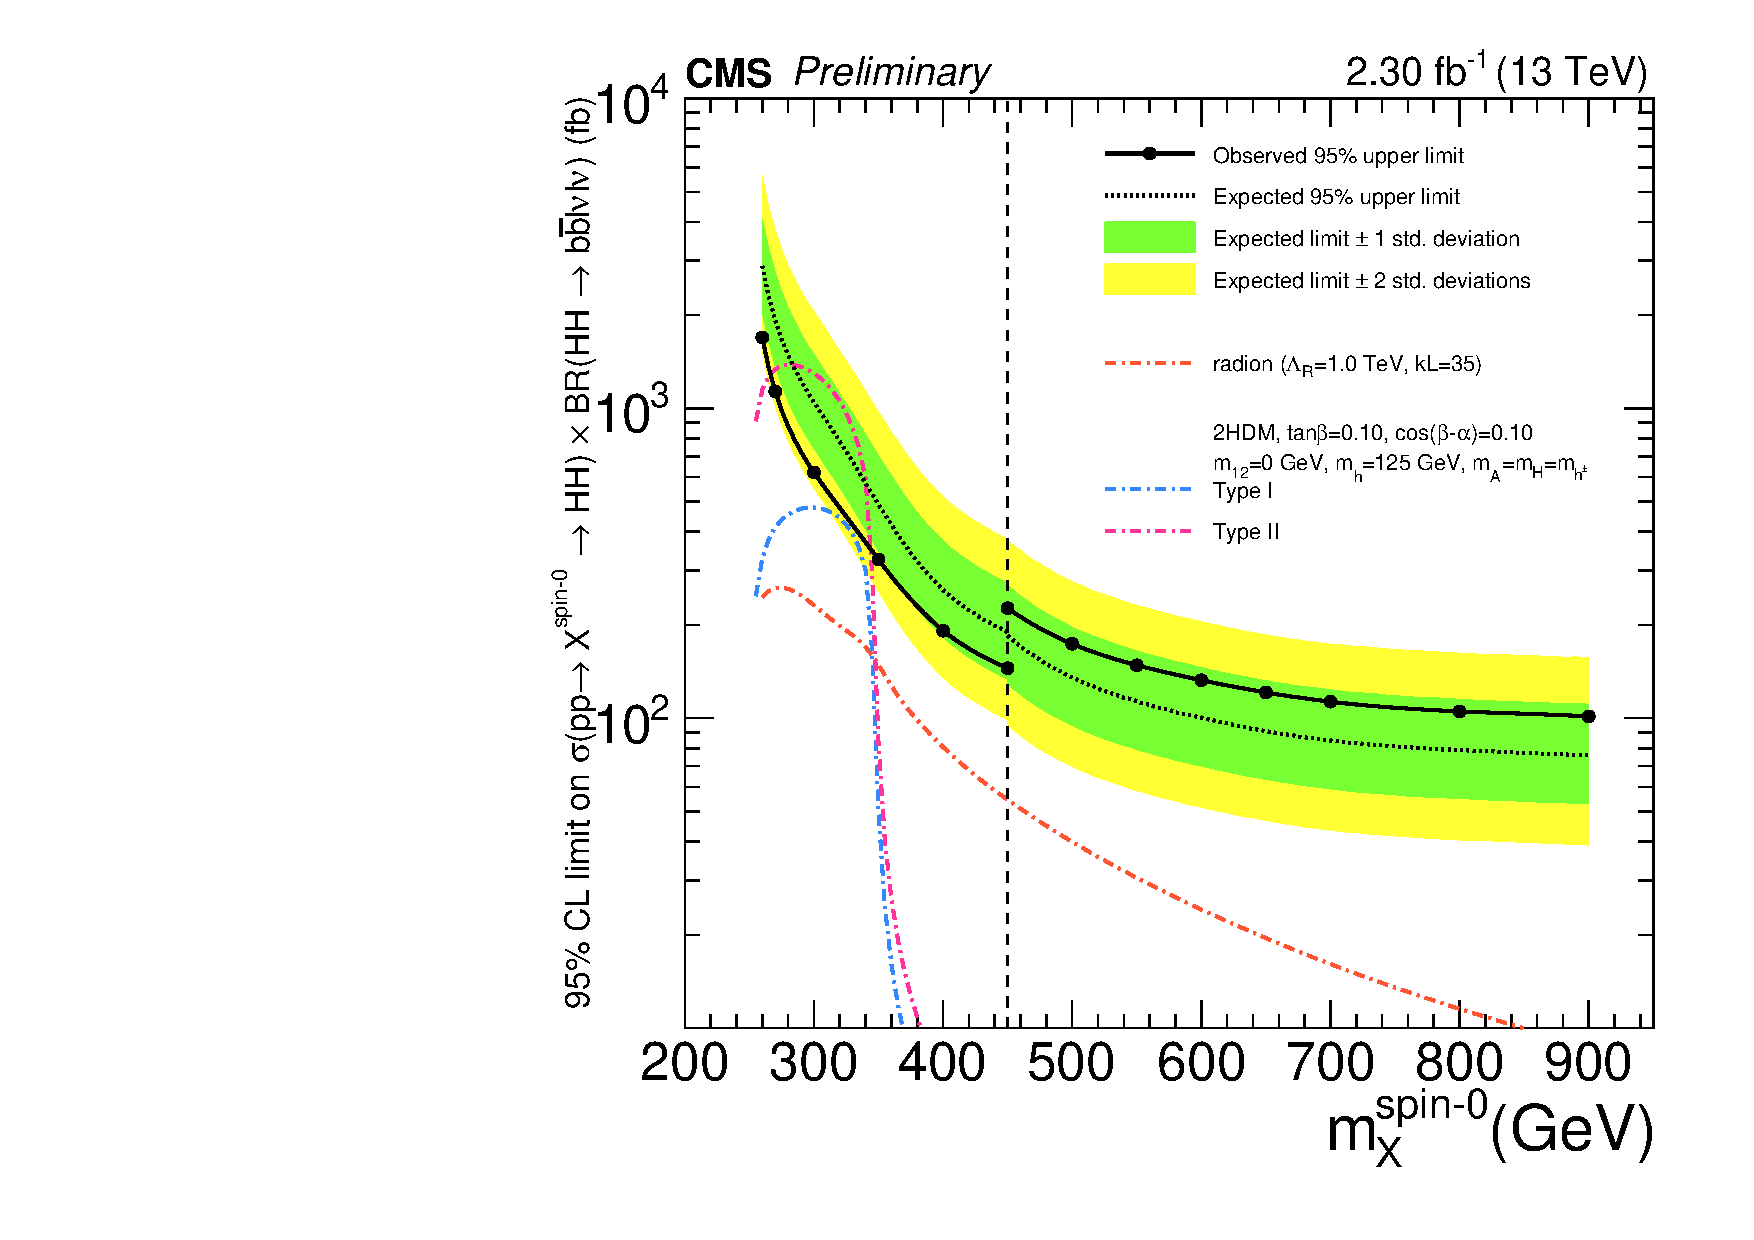
\includegraphics[width=0.5\textwidth, angle=0] {figures/H_hh_bbWW_CMS_BR.pdf}
\caption{Observed and expected 95\% CL upper limits on $\sigma(pp\rightarrow H) \times BR(H \rightarrow hh \rightarrow bbl\nu l\nu)$}
\label{fig:HH_bbWW}   
\end{figure}
%%

\subsection{$H\rightarrow hh \rightarrow bb\gamma\gamma$ channel}

The $bb\gamma\gamma$ final state is particularly promising for the DiHiggs search, as it benefits from the large branching fraction of the $h\rightarrow bb$ decay and the clean di-photon signal, due to high $m_{\gamma\gamma}$ resolution, on top of a smooth continuum di-photon background from multi-jet and multi-photon SM processes. 

The analysis performed by ATLAS collaboration scans masses in the range $275 GeV < m_H < 400 GeV$. A counting approach is adopted in order to estimate the number of signal and background events.

Observed and expected 95\% CL upper limits are shown in figure \ref{fig:HH_bbgg}.
 %%
\begin{figure}[htb]
\centering
	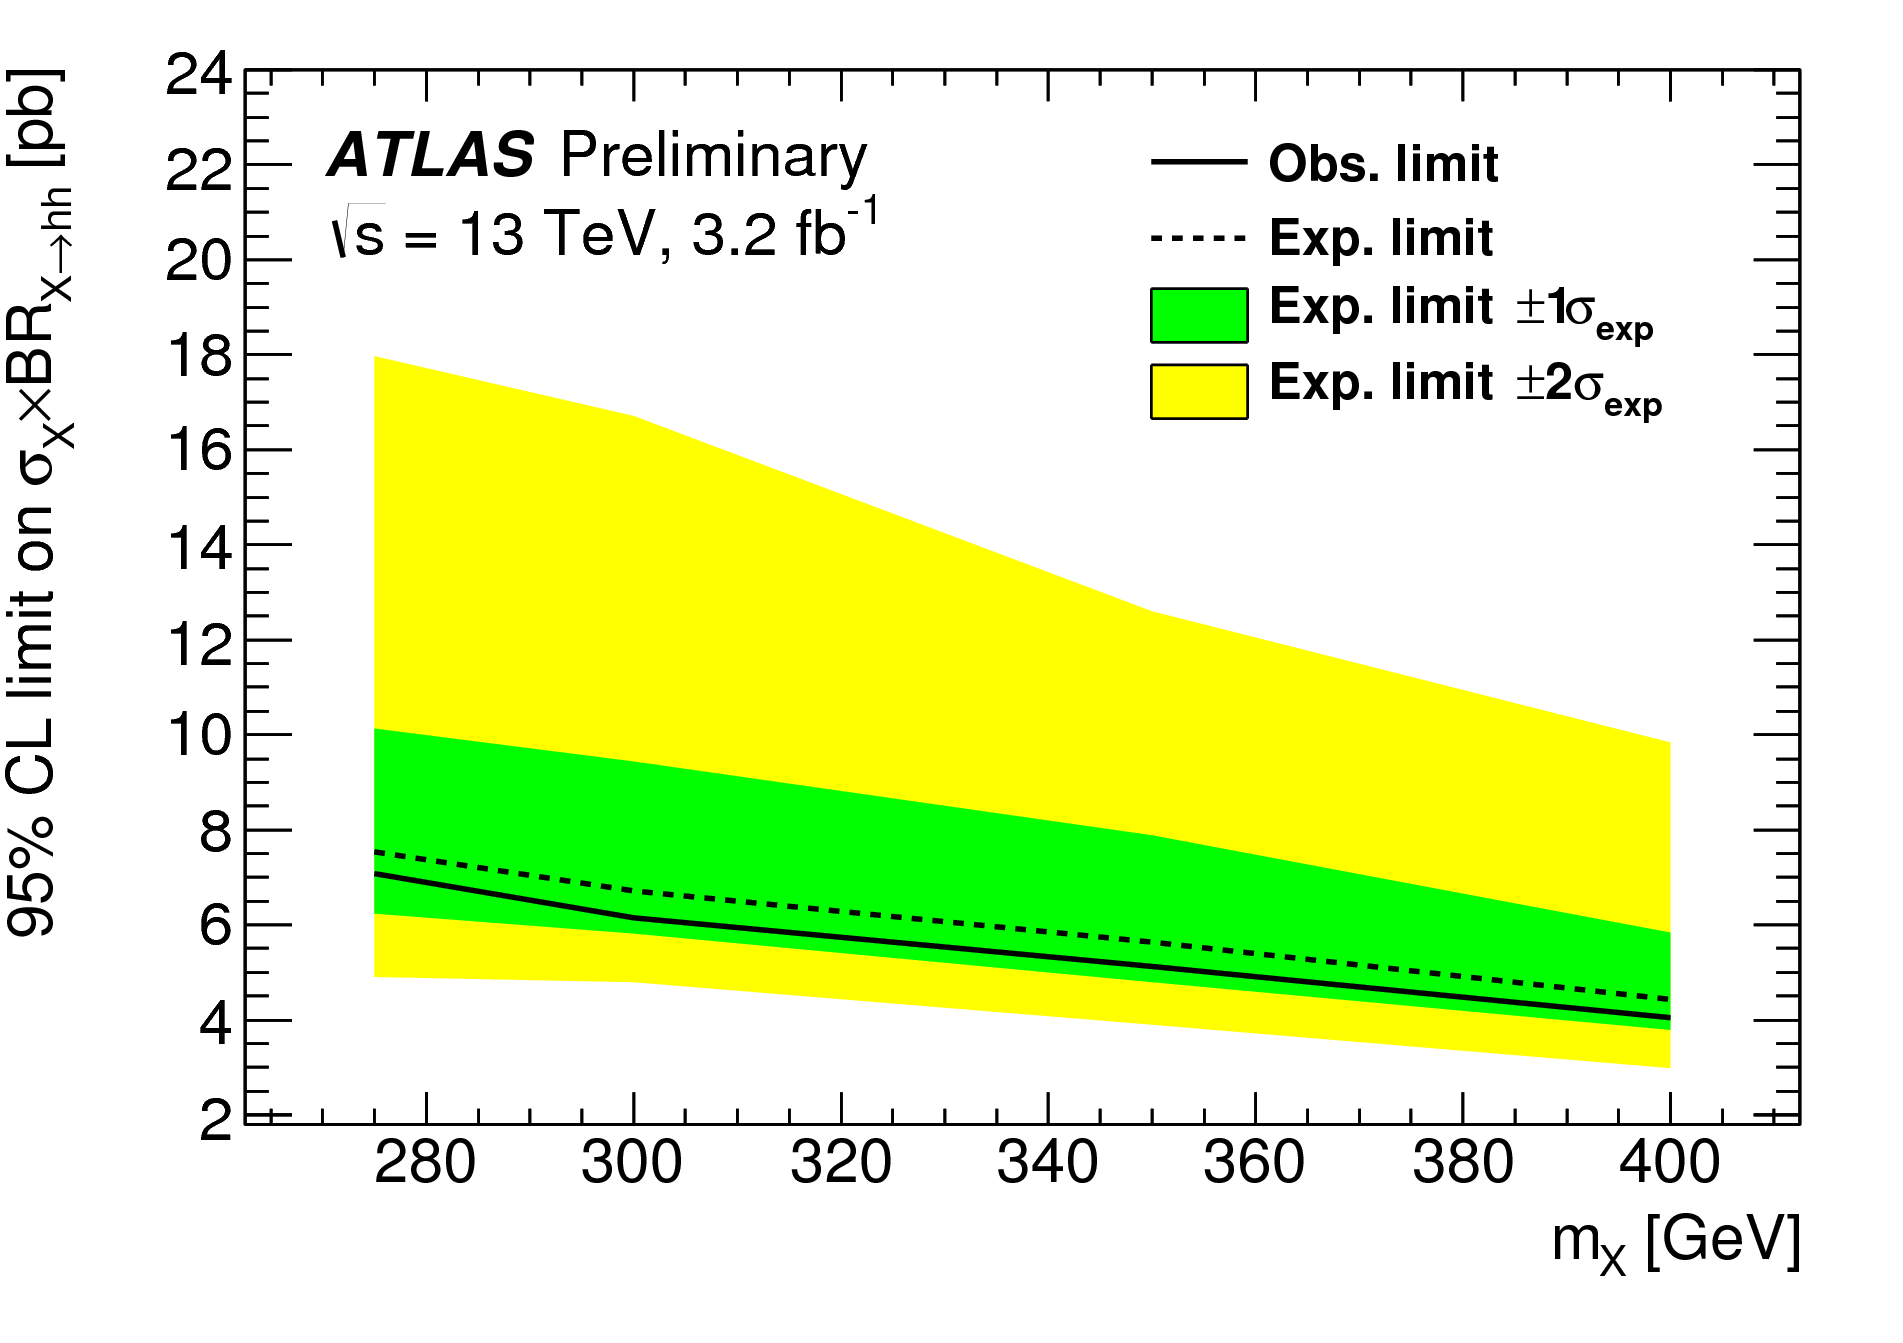
\includegraphics[width=0.6\textwidth, angle=0] {figures/H_hh_bbgg_ATLAS_BR.png}
\caption{Observed and expected 95\% CL upper limits on $\sigma(pp\rightarrow H) \times BR(H \rightarrow hh \rightarrow bb\gamma\gamma)$}
\label{fig:HH_bbgg}   
\end{figure}
%%







\newpage
\section{Conclusions}
The discovery of a scalar boson at the LHC
strengthened the interest for searches of extension of the scalar sector of the Standard Model.
A vast variety of searches have been performed by the ATLAS and CMS collaboration, using the data collected during the Run 1.  Thanks to proton-proton collisions at a center of mass energy of 13 TeV, the data collected in 2015 allowed the LHC collaborations to extend the reach in sensitivity in the searches for Higgs bosons beyond the SM. Searches for additional Higgs bosons performed so far have shown consistency with the SM predictions, although the data that will be collected in the next few years can enlighten the nature of the Higgs sector.

\begin{thebibliography}{99}
\bibitem{HH_ATLAS_8TeV} ATLAS Collaboration. \textsl{Searches for Higgs boson pair production in the $hh\ensuremath{\rightarrow}bb\ensuremath{\tau}\ensuremath{\tau}$, $\ensuremath{\gamma}\ensuremath{\gamma}W{W}^{*}$, $\ensuremath{\gamma}\ensuremath{\gamma}bb$, $bbbb$ channels with the ATLAS detecto}.
		\\10.1103/PhysRevD.92.092004, Phys. Rev. D, American Physical Society, 2015
\bibitem{HH_CMS_8TeV} \textsl{https://twiki.cern.ch/twiki/bin/view/CMSPublic/SummaryResultsHIG}.
\bibitem{...}
....

\end{thebibliography}

\end{document}
